\documentclass[a4paper]{article} 
\renewcommand{\thesubsection}{\thesection.\alph{subsection}}
\addtolength{\hoffset}{-2.25cm}
\addtolength{\textwidth}{4.5cm}
\addtolength{\voffset}{-3.25cm}
\addtolength{\textheight}{5cm}
\setlength{\parskip}{0pt}
\setlength{\parindent}{0in}

\usepackage[square,sort,comma,numbers]{natbib}
\usepackage{blindtext} % Package to generate dummy text
\usepackage{charter} % Use the Charter font
\usepackage[utf8]{inputenc} % Use UTF-8 encoding
\usepackage{microtype} % Slightly tweak font spacing for aesthetics
\usepackage{amsthm, amsmath, amssymb} % Mathematical typesetting
\usepackage{float} % Improved interface for floating objects
\usepackage{hyperref} % For hyperlinks in the PDF
\usepackage{graphicx, multicol} % Enhanced support for graphics
\usepackage{xcolor} % Driver-independent color extensions
\usepackage{pseudocode} % Environment for specifying algorithms in a natural way
\usepackage[yyyymmdd]{datetime} % Uses YEAR-MONTH-DAY format for dates

\usepackage{fancyhdr} % Headers and footers
\pagestyle{fancy} % All pages have headers and footers
\fancyhead{}\renewcommand{\headrulewidth}{0pt} % Blank out the default header
\fancyfoot[L]{} % Custom footer text
\fancyfoot[C]{} % Custom footer text
\fancyfoot[R]{\thepage} % Custom footer text
\newcommand{\note}[1]{\marginpar{\scriptsize \textcolor{red}{#1}}} % Enables comments in red on margin

%----------------------------------------------------------------------------------------

\usepackage{graphicx}

%-------------------------------
%	TITLE VARIABLES (identify your work!)
%-------------------------------

\newcommand{\yourname}{Ian Ma} % replace YOURNAME with your name
\newcommand{\yournetid}{s1743566} % replace YOURNETID with your NetID
\newcommand{\yourgp}{Group 12}
\newcommand{\assignmentnumber}{4} % replace X with assignment number

\begin{document}

%-------------------------------
%	TITLE SECTION (do not modify unless you really need to)
%-------------------------------
\fancyhead[C]{}
\hrule \medskip
\begin{minipage}{0.295\textwidth} 
\raggedright
\footnotesize
\yourname \hfill\\
\yournetid \hfill\\
\yourgp
\end{minipage}
\begin{minipage}{0.4\textwidth} 
\centering 
\large
Statistical Methodology\\ 
\large 
Hand-in  \assignmentnumber\\ 
\end{minipage}
\begin{minipage}{0.295\textwidth} 
\raggedleft
\today\hfill\\
\end{minipage}
\medskip\hrule 
\bigskip


%-------------------------------
%	ASSIGNMENT CONTENT (add your responses)
%-------------------------------

% Q1
\section{}
	Given:
		\[\begin{split}
			x &: \text{time spent for a crypto-mining}\\
			y &: \text{no. of crypto-coins mined by a novel device}
		\end{split}\]
	Where:
		\[\begin{split}
			x :& \text{ 73 82 14 56 43 47 85 86 24 33 19 66 68 51 40}\\
			 & \text{ 60 70 39 28 69 87 52 52 15 85 41 23 77 42 60}\\
			 y :& \text{ 34 42 0 28 15 20 50 30 0 8 15 20 40 20 6}\\
			 & \text{ 30 14 18 6 17 37 18 11 1 45 11 5 28 10 21}
		\end{split}\]
	
	\subsection{}
		A diagram is plotted using R:\\
			Code:
			\begin{verbatim}
				> x <- c(73,82,14,56,43,47,85,86,24,33,19,66,68,51,40,
					60,70,39,28,69,87,52,52,15,85,41,23,77,42,60)
				> y <- c(34,42,0,28,15,20,50,30,0,8,15,20,40,20,6,
					30,14,18,6,17,37,18,11,1,45,11,5,28,10,21)
				> plot(x,y)
			\end{verbatim}
		Plot:\\
			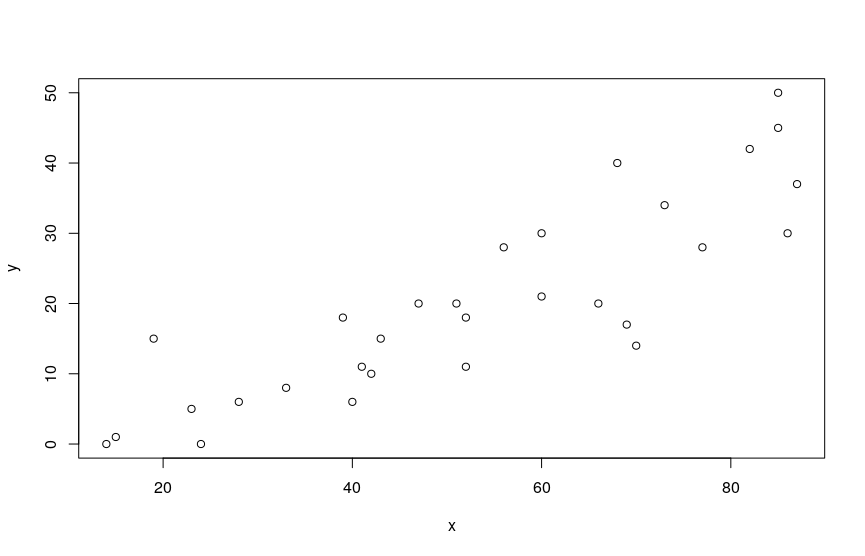
\includegraphics[width=\textwidth]{Rplot1A.png}
		Trend: There is a positiv relation between the time and number of mined crypto-coins, therefore the more the time spent, the more the crypto-coins mined.
	
	\newpage
	\subsection{}
		Assuming a simple linear regression is an appropriate model between \(x\) and \(y\) then:
			\\Let: \(y = \left\{y_1, y_2, ...\right\}\) where \(y_i \sim Y_i \forall i \in \mathbb{N}\) then:
			 \(\mathbb{E}(Y_i|x_i) = \beta_0 + \beta_1x_i\)
			 Where:
				\[\begin{cases}
					\begin{split}
						\hat{\beta_0} &= \bar{y} - \hat{\beta_1}\bar{x}\\
						\hat{\beta_1} &= \frac{\sum_i (x_i - \bar{x})y_i}{\sum_i (x_i - \bar{x})x_i} = S_{xy}/S_{xx}
					\end{split}
				\end{cases}\]
			Where:
				\[S_{xx} = \sum_i(x_i - \bar{x})^2\]
				\[S_{xy} = \sum_i(x_i - \bar{x})(y_i - \bar{y})\]
			With Using R:
				\begin{verbatim}
					> xbar = mean(x)
					> ybar = mean(y)
					> Sxx <- sum((x - xbar)^2)
					> Sxy <- sum((x-xbar)*(y-ybar))
					> beta_1 = Sxy/Sxx
					> beta_0 = ybar - beta_1*xbar
					> round(c(beta_0,beta_1),5)
					[1] -7.88777  0.52718
				\end{verbatim}
				We now know \(\hat{\beta_0} = -7.88777 \quad \hat{\beta_1} = 0.52718\)
			Therefore the least square estimate:
				\[\mathbb{E}(Y_i|x_i) = \hat{\beta_0} + \hat{\beta_1}x_i = -7.88777 + 0.52718x_i\]

	\newpage
	\subsection{}
		As we know:
		\[\begin{cases}
			\begin{split}
				\hat{\beta_0} &= \bar{y} - \hat{\beta_1}\bar{x}\\
				\hat{\beta_1} &= \frac{\sum_i (x_i - \bar{x})y_i}{\sum_i (x_i - \bar{x})x_i} = S_{xy}/S_{xx}
			\end{split}
		\end{cases}\]
		And Given: \(\hat{\sigma}^2 = \frac{1}{n-2}(S_{yy}-S_{xy}^2/S_{xx})\)\\
		Using R:
		\begin{verbatim}
			> Syy <- sum((y - ybar)^2)
			> n = 30
			> sigmaSquare = (Syy - Sxy^2/Sxx)/(n-2)
			> sigmaSquare
			[1] 49.74041
		\end{verbatim}
		We know that \(\hat{\sigma^2} = 49.74041\)\\
		Estimated Standard Error of \(\beta_1\):
			\begin{equation*}
				\begin{split}
					\sigma_{\beta_0}^2 &= Var(\hat{\beta_1}|\textbf{x}) = \frac{\sigma^2}{S_{xx}}\\
					\sigma_{\beta_0} &= \sqrt{\frac{\sigma^2}{S_{xx}}}
				\end{split}
			\end{equation*}
			\begin{equation*}
				\begin{split}
					\mathbb{E}(\sigma_{\beta_0}) &= \mathbb{E}\left(\sqrt{\frac{\sigma^2}{S_{xx}}}\right)\\
					&= 0.0579 \text{ }(4 \text{ d.p.})
				\end{split}
			\end{equation*}
		Estimated Standard Error of \(\beta_0\):
		\begin{equation*}
			\begin{split}
				\sigma_{\beta_1}^2 &= Var(\hat{\beta_0}|\textbf{x}) = \left(\frac{1}{n}+\frac{\bar{x}^2}{S_{xx}}\right)\sigma^2\\
				\sigma_{\beta_1} &= \sqrt{\left(\frac{1}{n}+\frac{\bar{x}^2}{S_{xx}}\right)\sigma^2}
			\end{split}
		\end{equation*}
		\begin{equation*}
			\begin{split}
				\mathbb{E}(\sigma_{\beta_0}) &= \mathbb{E}\left(\sqrt{\left(\frac{1}{n}+\frac{\bar{x}^2}{S_{xx}}\right)\sigma^2}\right)\\
				&= 3.3247 \text{ }(4 \text{ d.p.})
			\end{split}
		\end{equation*}
	\subsection{}
		When fitting the model, we have assumed \(\forall Y_i, i = 1,2,...\), all \(Y_i\):
			\begin{itemize}
				\item are uncorrelated
				\item have commoned variance \(\sigma^2\)
				\item have expectation \(\mathbb{E}(Y_i|x_i) = \beta_0 + \beta_1x_i\)
			\end{itemize}

\newpage
% Q2
\section{}
	Prove, for \(x_1, ..., x_n\) with mean \(\bar{x}\) and \(y_1, ..., y_n\) with mean \(\bar{y}\):
	\[
		\begin{split}
			S_{xx} = \sum_{i=1}^n(x_i-\bar{x})^2 \equiv \sum_{i=1}^n(x_i-\bar{x})x_i \equiv \sum_{i=1}^nx_i^n + n^{-1}\left(\sum_{i=1}^nx_i\right)^2\\
			S_{xy} = \sum_{i=1}^n(x_i-\bar{x})(y_i-\bar{y}) \equiv \sum_{i=1}^n (x_i - \bar{x})y_i \equiv \sum_{i=1}^nx_iy_i - n\bar{x}\bar{y}
		\end{split}
	\]
		Claim 1: \(S_{xx} = \sum_{i=1}^n(x_i-\bar{x})^2 \equiv \sum_{i=1}^n(x_i-\bar{x})x_i \equiv \sum_{i=1}^nx_i^n + n^{-1}\left(\sum_{i=1}^nx_i\right)^2\)\\
		Proof, direct proof:
			\begin{equation*}
				\begin{split}
					S_{xx} &= \sum_{i=1}^n(x_i-\bar{x})^2\\
					&= \sum_{i=1}^n(x_i-\bar{x})(x_i-\bar{x})\\
					&= \sum_{i=1}^n(x_i-\bar{x})x_i - \sum_{i=1}^n(x_i-\bar{x})\bar{x}\\
					&= \sum_{i=1}^n(x_i-\bar{x})x_i - \bar{x}\sum_{i=1}^n(x_i-\bar{x})\\
					&= \sum_{i=1}^n(x_i-\bar{x})x_i - \bar{x}\times 0\\
					&= \sum_{i=1}^n(x_i-\bar{x})x_i\\
				\end{split}
			\end{equation*}
			\[\therefore S_{xx} = \sum_{i=1}^n(x_i-\bar{x})^2 \equiv \sum_{i=1}^n(x_i-\bar{x})x_i\]
			\begin{equation*}
				\begin{split}
					S_{xx} &= \sum_{i=1}^n(x_i-\bar{x})x_i\\
					&= \sum_{i=1}^n \left(x_i^2 - x_i\bar{x}\right)\\
					&= \sum_{i=1}^n x_i^2 - \sum_{i=1}^nx_i\bar{x}\\
					&= \sum_{i=1}^n x_i^2 - \frac{1}{n}\sum_{i=1}^nx_i\sum_{i=1}^nx_i\\
					&= \sum_{i=1}^n x_i^2 - \frac{1}{n}\left(\sum_{i=1}^nx_i\right)^2
				\end{split}
			\end{equation*}
			\[\therefore S_{xx} = \sum_{i=1}^n(x_i-\bar{x})^2 \equiv \sum_{i=1}^n(x_i-\bar{x})x_i \equiv \sum_{i=1}^n x_i^2 - \frac{1}{n}\left(\sum_{i=1}^nx_i\right)^2\]
			\[\therefore \text{ claim true}\]
		Claim 2: \(S_{xy} = \sum_{i=1}^n(x_i-\bar{x})(y-\bar{y}) \equiv \sum_{i=1}^n (x_i - \bar{x})y_i \equiv \sum_{i=1}^nx_iy_i - n\bar{x}\bar{y}\)\\
		Proof, direct proof:
			\begin{equation*}
				\begin{split}
					S_{xy} &= \sum_{i=1}^n(x_i-\bar{x})(y_i-\bar{y})\\
					&= \sum_{i=1}^n(x_i-\bar{x})y_i - \sum_{i=1}^n(x_i-\bar{x})\bar{y}\\
					&= \sum_{i=1}^n(x_i-\bar{x})y_i - \bar{y}\sum_{i=1}^n(x_i-\bar{x})\\
					&= \sum_{i=1}^n(x_i-\bar{x})y_i - \bar{y} \times 0\\
					&= \sum_{i=1}^n(x_i-\bar{x})y_i
				\end{split}
			\end{equation*}
			\[\therefore S_{xy} = \sum_{i=1}^n(x_i-\bar{x})(y_i-\bar{y}) \equiv \sum_{i=1}^n(x_i-\bar{x})y_i\]
			\begin{equation*}
				\begin{split}
					S_{xy} &= \sum_{i=1}^n(x_i-\bar{x})y_i\\
					&= \sum_{i=1}^n \left(x_iy_i - \bar{x}y_i\right)\\
					&= \sum_{i=1}^n x_iy_i - \sum_{i=1}^n \bar{x}y_i\\
					&= \sum_{i=1}^n x_iy_i - n\bar{x}\frac{\sum_{i=1}^n y_i}{n}\\
					&= \sum_{i=1}^n x_iy_i - n\bar{x}\bar{y}
				\end{split}
			\end{equation*}
			\[\therefore S_{xy} = \sum_{i=1}^n(x_i-\bar{x})(y_i-\bar{y}) \equiv \sum_{i=1}^n (x_i - \bar{x})y_i \equiv \sum_{i=1}^nx_iy_i - n\bar{x}\bar{y}\]
			\[\therefore \text{ claim true}\]

\end{document}